\documentclass[11pt, a4paper]{COMP3711}
\usepackage{verbatim}
\usepackage{fancyhdr}
\usepackage{booktabs}
\usepackage{setspace}
\usepackage{amsmath,mathrsfs}
\usepackage{multicol}
\usepackage{amssymb}
\usepackage{graphicx}
\usepackage{caption}
\usepackage{subcaption}
\usepackage{array}
\usepackage{xcolor}
\usepackage{float}
\usepackage{enumitem}
\usepackage{mathcomp}
\usepackage{tabularx}
\usepackage{wasysym}
\usepackage{pbox}
\usepackage{tikz}
\usepackage{mathtools}
\usepackage{hyperref}
\hypersetup{hidelinks}
\usetikzlibrary{matrix}
\usepackage[normalem]{ulem}
\usepackage{multirow}
\usepackage[linesnumbered, ruled, boxed]{algorithm2e}
\SetKwRepeat{Do}{do}{while}

\title{Topic 2}
\subtitle{Divide \& Conquer}

\begin{document}
\begin{spacing}{1.5}
    
    \section{Intro: Binary Search}

    The main idea of {\rm Divide \& Conquer} is to solve a problem(such as of 
    size $n$) by breaking it into one or more smaller(size less than $n$) problems.
    We use binary search example to illustrate that.

    {\bf Problem:} given an {\bf sorted} array of length $n$, how to find 
    the position of element $x$; if $x$ does not exist
    in the array, output nil.

    Since the array is already sorted, it has a good property that:
    {\bf for each item $a_i$, those who are larger than $a_i$ must be 
    on its right side, while smaller than $a_i$ must be on its left side.}
    Hence we come up with an idea that we check the middle item $mid$ first,
    then we will be able to know which direction to go: left or right,
    depending on the comparison of $mid$ and $x$(the item we're looking for).
    If we go left, then the right half will be directly abandoned.
    Then we continue this process, check middle item each time, and 
    abandon half items each time.

    \begin{algorithm*}
        \caption{BinarySearch($a[]$, $left$, $right$, $x$)}
        \KwData{$a[]$: the array given, $x$: the item to find}
        \eIf{$left=right$}{
            \eIf{$a[left]=x$}{
                return $left$
            }{
                return {\bf nil}
            }
        }{
            $mid=\lfloor (left + right) / 2\rfloor$

            \eIf{$x\le a[mid]$} {
                BinarySearch($a[]$, $left$, $mid$, $x$)
            }{
                BinarySearch($a[]$, $mid+1$, $right$, $x$)
            }
        }
    \end{algorithm*}

    {\bf First call:} BinarySearch($a[]$, 1, $n$, $x$).

    This algorithm is quite efficient, since each time 
    we eliminate half of the array, with one additional 
    comparison, until there is only one item left,
    when we will end the process.

    Then let's analyse its time complexity. Let $T(n)$ be the number of 
    comparisons needed for $n$ elements, then we will have
    $$T(n)=T(n/2)+1,\ T(1)=1$$.

    Solve this {\bf recurrence}:
    \begin{align*}
        T(n) &= T(n/2) + 1\\
            &= [T(n/4) + 1] + 1\\
            &= T(n/4) + 2\\
            &=\cdots\\
            &=T(n/2^{i}) + i
    \end{align*}

    This process ends when reaching $T(1)$, i.e., 
    $i=\log_2 n$, thus, $T(n)=T(1)+\log_2 n=\log_2 n + 1$.

    We can also visualize this recurrence with recursion tree:
    (image from lecture note)
    \begin{center}
        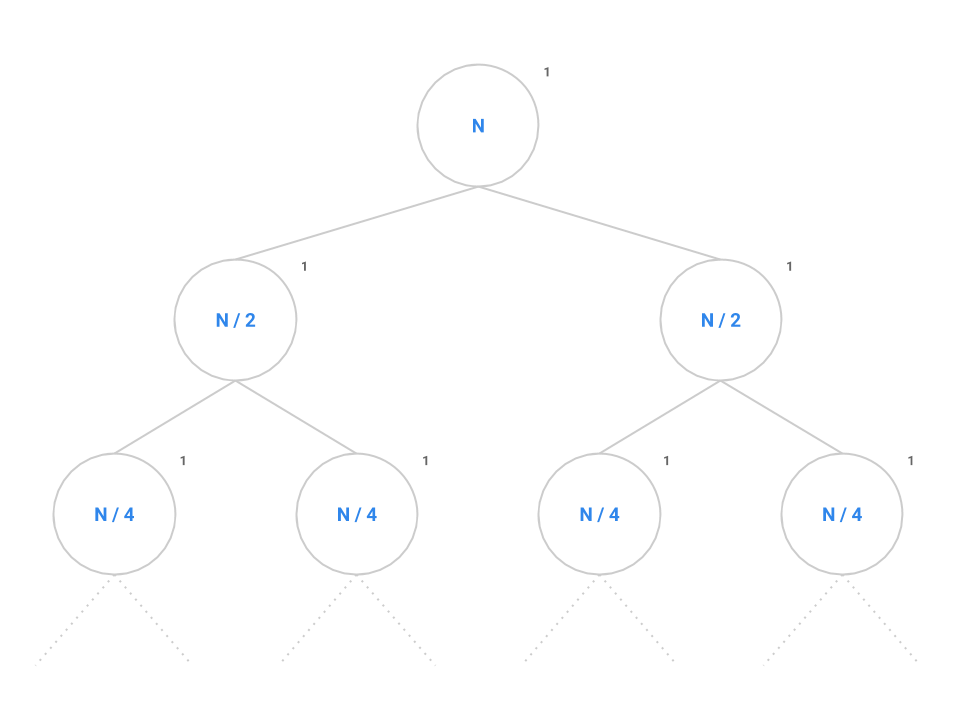
\includegraphics[scale=0.35]{images/02-bs-tree.png}
    \end{center}

    In each recursion step(level), we use 1 comparison(compare 
    $mid$ and $x$), then call recursion on a half 
    of the original array. From the image above, 
    we can easily notice there are total 
    $1+1+\cdots+1=1+\log_2 n$ comparisons.

    \section{Example: Towers of Hanoi}

    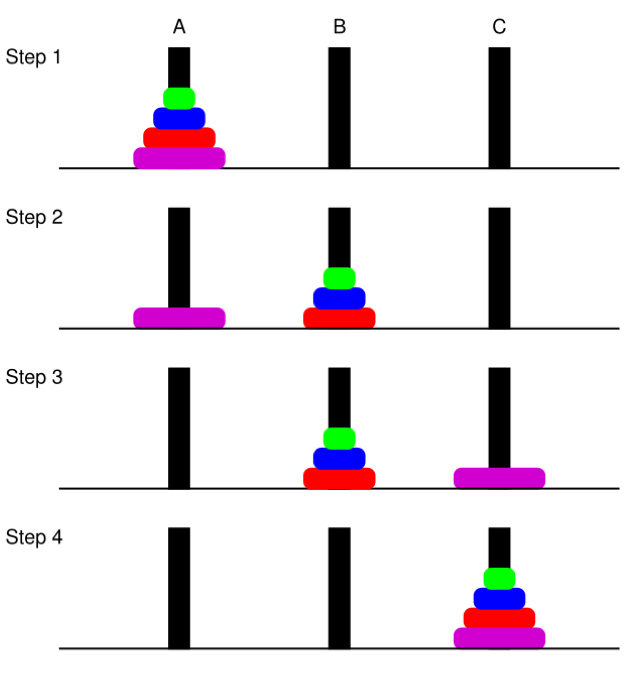
\includegraphics[scale=0.28]{images/02-hanoi.jpeg}
    
    In this example, we want to design an algorithm to 
    move all $n$ discs from peg $A$(start) to peg $C$(end), with the 
    constraints: (1) move one disc at a time, and 
    (2) cannot put larger disc on a smaller one.
    We are given another peg $B$(helper) where we can 
    temporary storage our discs.

    We still use the idea of {\bf Divide \& Conquer},
    consider how we can turn a problem of $n$ discs 
    into a problem of $n-1$? One possible solution is that,
    we can call recursion on upper $n-1$ discs, i.e., 
    move upper $n-1$ discs to peg $B$(helper peg), then move the remaining
    (the biggest) disc to peg $C$(end peg), and finally 
    move the $n-1$ discs from peg $B$(helper) to peg $C$(end).
    The following pseudocode shows this idea.

    \begin{algorithm*}
        \caption{MoveTower($n$, $start$, $helper$, $end$)}
        \KwIn{$n$: num of discs}
        \eIf{$n=1$}{
            move the only disc from $start$ peg to $end$ peg

            return
        }{
            {\tcp {move first $n-1$ from $start$ peg to $helper$ peg}}
            {\tcp {so this time ``helper'' peg will be the old $end$ peg}}
            {\bf MoveTower($n-1$, $start$, $end$, $helper$)}

            move the only disc from $start$ peg to $end$ peg

            {\tcp {finally move first $n-1$ from $helper$ peg to $end$ peg}}
            {\tcp {this time ``helper'' peg will be the old $start$ peg}}
            {\bf MoveTower($n-1$, $helper$, $start$, $end$)}
        }
    \end{algorithm*}

    Now we would like to analyze the time complexity of this algorithm,
    in other words, how many {\bf steps} are needed.
    Let $T(n)$ be the num of steps for $n$ discs, each time, 
    we first move $n-1$ disks from $start$ to $helper$, 
    costs $T(n-1)$ steps; then we move the biggest disk to $end$ peg,
    costs only 1 step; finally we move $n-1$ disks from $helper$
    to $end$, again costs $T(n-1)$ steps. To sum up:
    $$T(n)=2T(n-1)+1$$ when $n>1$, and $T(1)=1$.

    Now we solve the recurrence by the {\bf expansion method}:
    \begin{align*}
        T(n) &= 2T(n-1) + 1\\
             &= 2[2T(n-2)+1] + 1\\
             &= 4T(n-2)+3\\
             &= 4[2T(n-3)+1] + 3 \\
             &= 8T(n-3) + 7\\
             &= \cdots \\
             &= 2^i T(n-i) + (2^i-1)\\
             &= 2^{n-1} T(1) + (2^{n-1}-1)\\
             &= 2^n-1
    \end{align*}

    Or, with the recursion tree method:
    \begin{center}
        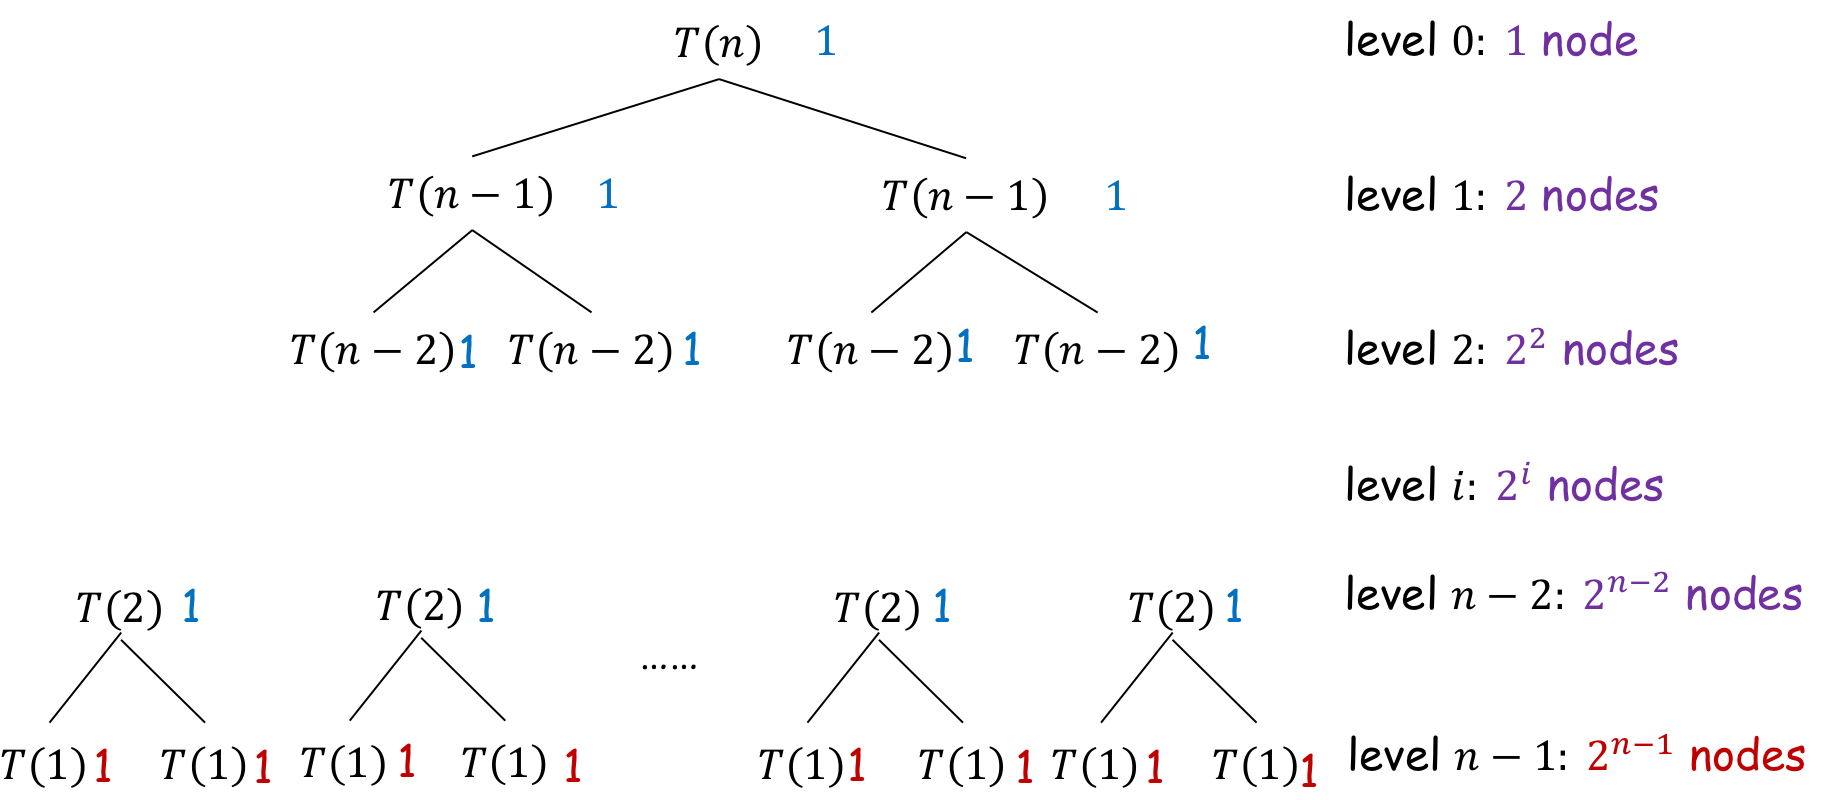
\includegraphics[scale=0.2]{images/02-hanoi-tree.jpeg}
    \end{center}
    
    There are, altogether, $1+2+2^2+2^3+\cdots + 2^{n-2}+2^{n-1}
    =2^n-1$ nodes, and we are doing one work(step) each node,
    then the time complexity is again, $2^n-1$.

    \section{Merge Sort}

    Now we again back to sorting, and we would like to introduce 
    a new algorithm or sorting: Merge Sort.
    This is a typical example of divide \& conquer, and 
    its process is like: (1) we first divide array into two halves,
    (2) then we recursively sort each half, (which means we 
    continuously divide it into halves, and then halves...)
    (3) finally {\bf merge} two halves to get a whole.

    The {\bf merge} operation may confuse you most. Here 
    it means combine two {\bf sorted lists} into a 
    whole sorted list. For example, given two sorted lists:
    $A=[2, 5, 7]$ and $B=[3, 4, 6, 10, 12]$, then after {\bf merge}
    operation, we will get $result=[2, 3, 4, 5, 6, 7, 10, 12]$.
    Since these two lists are sorted, we can do this process
    in $O(n)$ time, where $n$ is the length of result 
    list.(how many numbers in total) The basic idea is: 
    we compare the first item of $A$ and $B$, put the smaller 
    one, say, $A[1]$, in the first position of result list, then 
    we move on to the next item of $A$, but compare it still with 
    the {\bf first} item of $B$(since the first item of $B$
    has not yet inserted into result list), 
    and again put the smaller one into result list, then 
    continue move on. An example may help you understand the process:

    (1) Compare first items: $A=[{\blue 2},5,7], B=[{\blue 3},4,6,10,12]$, 
    $2<3$, so $result=[2]$;

    (2) then compare 2nd in $A$ and 1st in $B$, $A=[2, {\blue 5},7], B=[{\blue 3},4,6,10,12]$, 
    $3<5$, so $result=[2, 3]$;

    (3) continue the process, similarly, $A=[2, {\blue 5},7], B=[3,{\blue 4},6,10,12]$, 
    $4<5$, so $result=[2, 3, 4]$;

    (4) $A=[2, {\blue 5},7], B=[3,4,{\blue 6},10,12]$, 
    $5<6$, so $result=[2, 3, 4, 5]$;

    (5) $A=[2, 5,{\blue 7}], B=[3,4,{\blue 6},10,12]$, 
    $6<7$, so $result=[2, 3, 4, 5, 6]$;

    (6) $A=[2, 5,{\blue 7}], B=[3,4,6,{\blue 10},12]$, 
    $7<10$, so $result=[2, 3, 4, 5, 6, 7]$;

    (7) Now, all items in $A$ have already been inserted into result 
    list so that no items can be compared with items in $B$.
    Then we simply add remaining items in $B$ to result list,
    this will, obviously, ensure a sorted result list.(you may think of why)
    Hence $result=[2,3,4,5,6,7,{\blue 10,12}]$

    The pseudocode below shows the process:
    (below, append $\infty$ at the end of two lists can 
    free us from considering the situation that one list is 
    empty, like (7) above. Though different implementation, 
    the idea is entirely the same)
    
    \begin{algorithm*}
        \caption{Merge($A$, $left$, $mid$, $right$)}
        \tcp{merge two sorted list: $A[left\cdots mid]$ and $A[mid+1\cdots right]$}
        $L\lar A[left\cdots mid],\ R\lar A[mid+1\cdots right]$

        append $\infty$ at the end of $L$ and $R$ \qquad \tcp{see explanation above}

        $i\lar 1,\ j\lar 1$\qquad  \tcp{two pointers point at items in $L$ and $R$}

        \For{$k\lar left$ {\rm to} $right$} {
            \tcp{always choose the smaller one to insert, and move on}
            \eIf{$L[i] \le R[j]$}{
                $A[k]\lar L[i]$

                $i\lar i + 1$
            }{
                $A[k] \lar R[j]$

                $j\lar j + 1$
            }
        }
    \end{algorithm*}

    After learning how {\bf Merge} works, you now, hopefully,
    are able to understand how Merge Sort works, with the image below:

    \begin{center}
        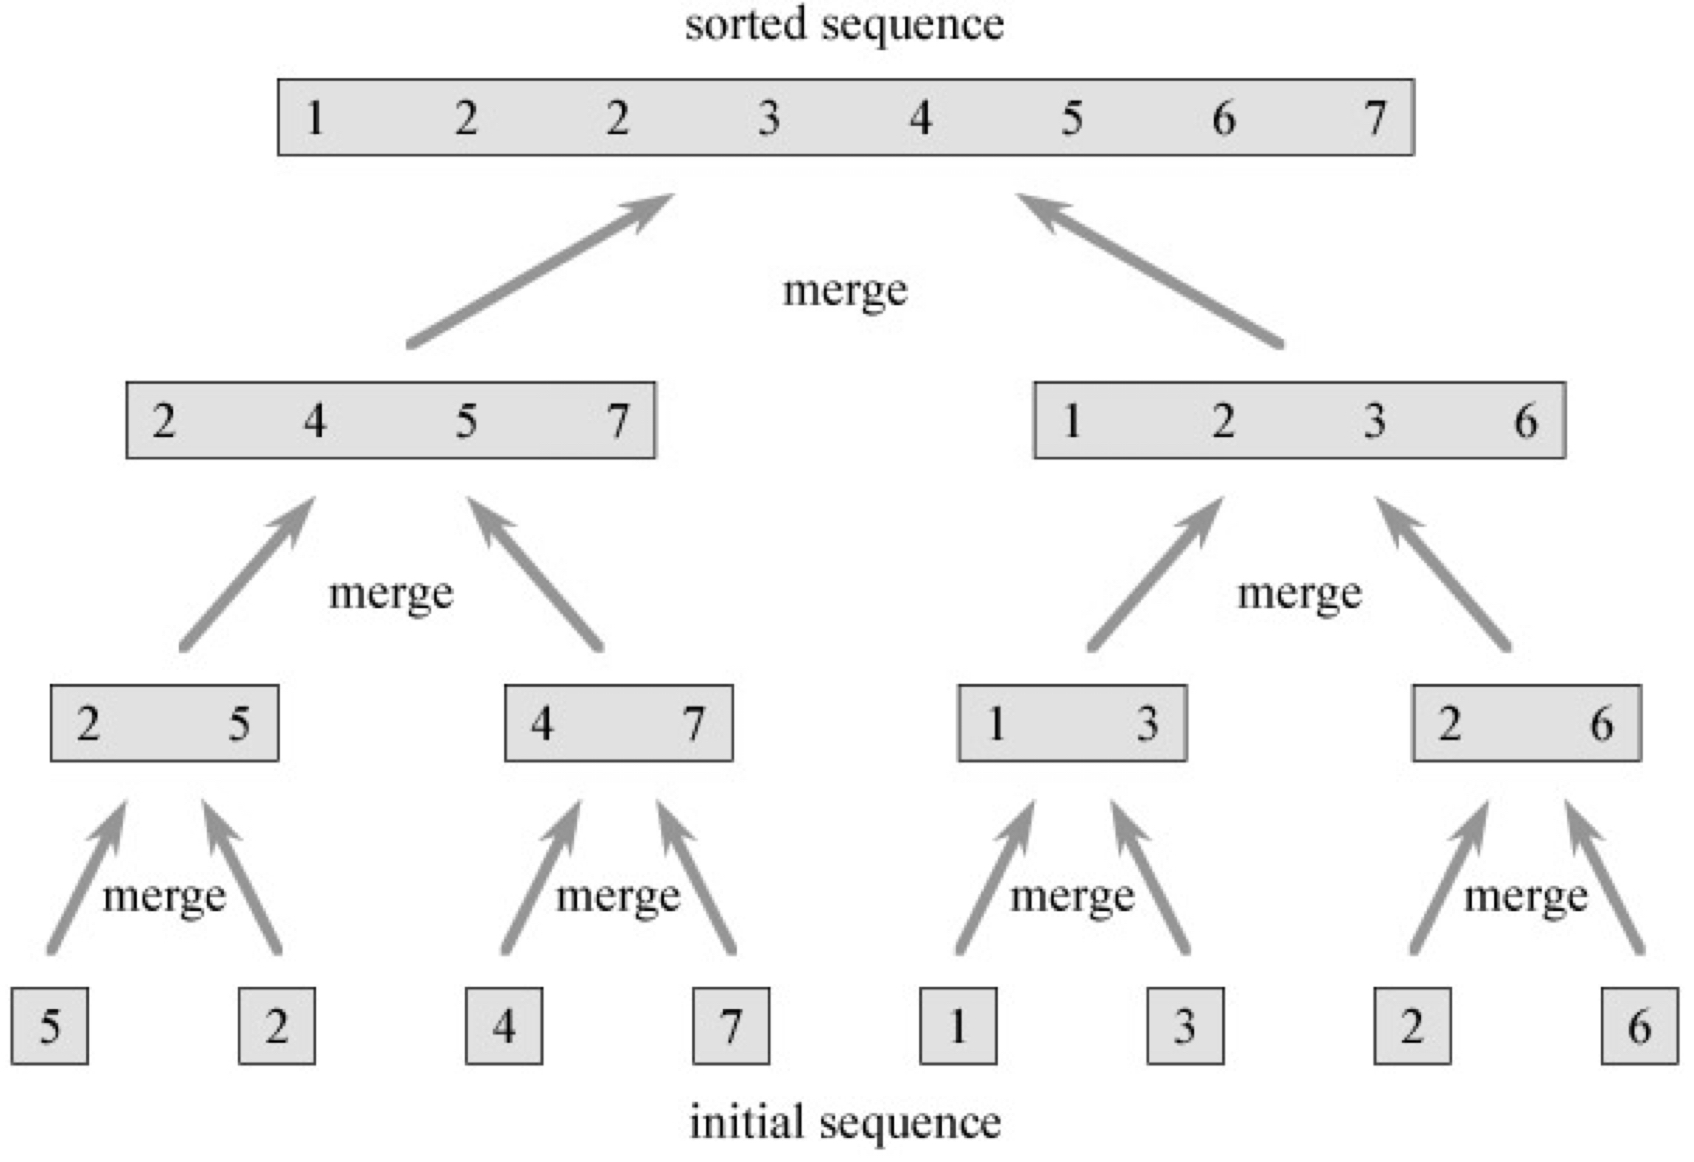
\includegraphics[scale=0.2]{images/02-mergeSort.jpeg}
    \end{center}
    
    We break down array recursively, until one element left,
    and then merge from bottom to up.
    The complete pseudocode for Merge Sort is given below:
    \begin{algorithm*}
        \caption{MergeSort($A$, $left$, $right$)}
        \If{$left=right$}{return}
        $mid\lar \lfloor (left + right) / 2 \rfloor$

        \tcp{recursively divide array into two halves}

        {\bf MergeSort($A$, $left$, $mid$)}

        {\bf MergeSort($A$, $mid+1$, $right$)}

        \tcp{then merge from bottom to up}

        {\bf Merge($A$, $left$, $mid$, $right$)}
    \end{algorithm*}

    Firstly call {\bf MergeSort($A$, 1, $n$)} to sort array $A$.
    
    As usual, we are interested in the running time of Merge Sort 
    algorithm. Let $T(n)$ be the running time on an array of size $n$,
    it's not hard to find 
    $T(n)\le T(\lfloor n/2 \rfloor) + T(\lceil n/2 \rceil)+O(n)$,
    when $n>1$ and $T(1)=O(1)$.

    Here we are actually able to simplify the equation. Firstly 
    we can replace $\le $ with $=$, since we are insterested
    in big-$O$ upper bound of $T(n)$; and with the same 
    reason, we can replace $O(n)$ with $n$, $O(1)$ with 1;
    finally, we can assume $n$ is a power of 2 for the sake of 
    simplicity but doesn't change the result at all, as 
    $T(n)\le T(n')\le T(2n)=O(T(n))$ where $n'$ is the 
    smallest power of 2 such that $n'\ge n$.

    Now we want to solve: 
    $T(n)=2T(n/2)+n$ for $n>1$, and $T(1)=1$.
    \begin{align*}
        T(n) &= 2\left(\frac{n}{2}\right)+n\\
             &= 2\left[ 2T\left(\frac{n}{4}\right) +\frac{n}{2}\right] + n
              = 2^2\cdot T\left(\frac{n}{2^2}\right) +2n\\
             &= 2^2\cdot \left[ 2T\left(\frac{n}{2^3}\right) +\frac{n}{2^2}\right] + 2n
              = 2^3\cdot T\left(\frac{n}{2^3}\right) +3n\\
             &= \cdots\\
             &= 2^{k}\cdot T\left(\frac{n}{2^k}\right) +kn
    \end{align*}
    We know the process ends with $\dfrac{n}{2^k}=1$ i.e. $k=\log_2 n$, thus
    \begin{align*}
        T(n) &= 2^{\log_2 n}T\left(\frac{n}{2^{\log_2 n}}\right)+n\cdot \log_2 n\\
             &= n\log_2 n+n
    \end{align*}
    In summary, merge sort runs in $O(n\log n)$ time.
    It is also worth pointing out that merge sort {\bf always}
    runs in $O(n\log n)$ time, which means best case is the same 
    as worst case, as you may think of it, 
    the complexity of merge sort {\it does not depend on inputs},
    it always break array down and then merge up.

    \section{Inversion Numbers}

    Given an array $A[1\cdots n]$, we say two elements $A[i]$ and $A[j]$
    are {\bf inverted} if $i<j$ but $A[i]>A[j]$, i.e., $A[i]$ appears
    before $A[j]$ but is larger than $A[j]$. The number of inverted pairs
    is called the {\bf inversion number} of array $A$. 
    Actually this is a useful measure, it provides us with an intuitive
    idea about how ``sorted'' an array is, larger inversion number implies
    a more unsorted array.

    What may surprise you is that inversion number has a close relation
    to insertion sort, and more concretely, {\bf the number of swaps
    used by insertion sort is equals to inversion number.}
    We can prove it by induction:
    
    \begin{proof}
        Assuming the array has size $n$. Basic case
        $n=2$ obviously holds.

        Inductive step: assume correct for an array of size $n-1$, i.e.,
        the total number of swaps performed while insertion sorting
        $A[1\cdots n-1]$ is equals to the inversion number of $A[1\cdots n-1]$.

        Let $x=A[n]$. Now, the remaining work by insertion sort is that we swap 
        $x$ with all items $A[j]$ such that $j<n$ and $A[j]>x$, 
        notice that the number of those items is the same of inversions in which
        {\bf $x$ participates}. Therefore, adding these new inversions gives
        the full inversion number of $A[1\cdots n]$.
    \end{proof}

    Now we will consider how to compute the inversion number of a given 
    array with size $n$. One possible method is we check all $(i,j)$
    pairs of given array, this requires ${n\choose 2}=\Theta(n^2)$
    running time. Another method uses the relation we proved above,
    running insertion sort and count the number of swaps we perform,
    but this also requires $\Theta(n^2)$ time since insertion sort 
    requires $\Theta(n^2)$. How can we improve that? 
    Come back to topic: divide and conquer!

    Similar to previous problems, we divide array into two halves, 
    and recursively count inversions in each half, but notice:
    we are missing something: we still need to count inversions
    where $a_i$ and $a_j$ are in different halves! We need 
    to return the sum of those three quantities finally.

    So the main problems is that, how we count the third quantity?
    Consider below situation, the two halves of array are:
    $[1,5,4,8,10,2]$ and $[6,9,12,11,3,7]$, how would you do that?
    You may count by hand, and knowing there are $5-3, 4-3, 8-6, \cdots$
    and in total 9 inversions with one item in 1st array and another in 
    2nd. But, it's really time consuming and totally a mess! We have 
    no efficient algorithm to do this but count one by one.

    But, things will become much better if those two arrays are 
    {\it sorted}. For example, $A=[3,7,10,14,18,19]$ and 
    $B=[2,11,16,17,23,25]$. How will we do then? We can 
    scan progressively through both lists, and for each item 
    in $B$, we only need to find the smallest $A$ item 
    larger than it. In the lists above, for example, $A[1]=3$
    is larger than $B[1]=2$, so all items in $A$ form an inversion pair 
    with $B[1]$; then we move to $B[2]=11$, we try to find the smallest 
    item in $A$ larger than 11, so we move the pointer in $A$, 
    $A[2]=7<11, A[3]=10<11$, until $A[4]=14>11$, so 
    each item in $A[4]\cdots A[6]$ can form an inversion pair with $B[2]$.
    If we continue the process, we will finally get the inversion 
    number formed between $A$ and $B$, in $O(n)$ time. (Why is $O(n)$?
    Since we only iterate each item once during the whole process.
    You may find it quite similar to Merge operation in Merge Sort)

    \begin{algorithm*}
        \caption{Count($A$, $l$, $mid$, $r$)}
        $L\lar A[l\cdots mid],\ R\lar A[mid+1\cdots r]$

        (here assume) $L, R$ already sorted

        $i\lar l,\ j\lar mid+1$\qquad \tcp{two pointers for $L$ and $R$}

        $ans\lar 0$ \qquad \tcp{total inversion number}

        \tcp{let $i,j$ iterator over two arrays}
        \While{$i\le mid$ and $j\le r$}{
            \tcp{looking for smallest $L$ item larger than $R$}
            \eIf{$L[i]\le R[j]$}{ 
                $i\lar i+1$
            }{
                \tcp{Found $L[i] > R[j]$!}

                \tcp{then $L[i]\cdots L[mid]$ each can form an inversion pair with $R[j]$}

                \tcp{so inversion num for $R[j]$ is $mid-i+1$}

                $inv\lar (mid-i+1)$

                $ans\lar ans+inv$

                $j\lar j+1$
            }
        }
        return $ans$
    \end{algorithm*}
\end{spacing}
\end{document}
